\documentclass{report}
\usepackage{graphicx} % Required for inserting images
\usepackage[english]{babel}
\usepackage{amsthm}
\usepackage{amsmath}
\usepackage{amsfonts}
\usepackage{tikz}
\usetikzlibrary{matrix}
\usepackage[english]{babel}
\usepackage{mathtools}

\title{MMath project}
\author{Saxon Supple }
\date{January 2024}

\newtheorem{definition}{Definition}
\newtheorem{lemma}{Lemma}
\newtheorem{theorem}{Theorem}
\newtheorem{proposition}{Proposition}
\newtheorem{corollary}{Corollary}

\begin{document}

\maketitle

\section{Singular homology}
\begin{definition}
A \textbf{k-simplex} is the convex hull\\
$[v_0,...,v_k]:=\{\sum_{i=0}^k\lambda_iv_i:\lambda_i\in [0,1],\sum_{i=0}^k\lambda_i=1\}$\\
of $k+1$ linearly independent vectors $v_0,...,v_k\in\mathbb{R}^n$.\\
The \textbf{standard k-simplex} is\\$\Delta^k=[e_0,...,e_k]=\{(t_0,...,t_k)\in\mathbb{R}^k:t_i\geq 0, \sum_{i=0}^kt_i=1\}$\\
The vectors $v_0,...,v_k$ define a \textbf{framing} $F_{v_0,...,v_k}\colon\Delta^k\rightarrow [v_0,...,v_k],(t_i)\mapsto \sum_{i=0}^kt_iv_i$.
\end{definition}


\noindent For example $\Delta^0$ is a point, $\Delta^1$ a line segment, $\Delta^2$ a triangle and $\Delta^3$ a tetrahedron.

\begin{definition}
The \textbf{faces} of $[v_0,...,v_k]$ are the (k-1)-simplices $[v_0,...,\overset{\wedge}{v_i},...,v_k]$ where $\overset{\wedge}{v_i}$ means omit the entry $v_i$.
\end{definition}

\begin{definition}
Let $X$ be a topological space. A \textbf{singular k-simplex} in X is a continuous map $\sigma\colon\Delta^k\to X$. The \textbf{k-th chain group} of $X$ is the abelian group\\
$C_k(X):=\{\sum_{i=1}^kn_i\sigma_i:k\in\mathbb{N}_0,n_i\in\mathbb{Z},\sigma_i \text{ is a k-simplex}\}$ where the elements are called \textbf{k-chains}.
\end{definition}

\begin{definition}
The \textbf{boundary map} $\partial=\partial_k\colon C_k(X)\to C_{k-1}(X)$ is given by\\
$\partial\sigma=\sum_{i=0}^k(-1)^i\sigma\circ F_{e_0,...,\overset{\wedge}{e_i},...,e_k}\in C_{k-1}(X)$\\
on single simplices and extended linearly to all of $C_k(X)$.
\end{definition}
\noindent Intuitively this definition means that the boundary map decomposes $\sigma$ into a sum of maps to its faces--or rather the images of faces of $\Delta^k$--taking into account orientation.


\begin{lemma}
$\partial\circ\partial\colon C_k(X)\to C_{k-2}(x)$ is zero.
\end{lemma}
\begin{proof}
Let $\sigma\in C_k(X)$.\\
$\partial\circ\partial (\sigma)=\partial(\sum_{i=0}^k(-1)^i\sigma\circ F_{e_0,...,\overset{\wedge}{e_i},...,e_k})$\\
$=\sum_{i=0}^k(-1)^i\partial\circ\sigma\circ F_{e_0,...,\overset{\wedge}{e_i},...,e_k}$ by linearity\\
$=\sum_{i=0}^k(\sum_{j<i}(-1)^{i+j}\sigma\circ F_{e_0,...,\overset{\wedge}{e_j},...,\overset{\wedge}{e_i},...,e_k} + \sum_{i<j}(-1)^{i+j-1}\sigma\circ F_{e_0,...,\overset{\wedge}{e_i},...,\overset{\wedge}{e_j},...,e_k})$ (since $e_j$ gets shifted forward one spot when $e_i$ is removed first)\\
$=\sum_{i=0}^k(\sum_{j<i}(-1)^{i+j}\sigma\circ F_{e_0,...,\overset{\wedge}{e_j},...,\overset{\wedge}{e_i},...,e_k} + \sum_{j<i}(-1)^{i+j-1}\sigma\circ F_{e_0,...,\overset{\wedge}{e_j},...,\overset{\wedge}{e_i},...,e_k})$
(interchanging $j$ with $i$ in the second term)\\
$=\sum_{i=0}^k(\sum_{j<i}((-1)^{i+j}+(-1)^{1+j-1})\sigma\circ F_{e_0,...,\overset{\wedge}{e_j},...,\overset{\wedge}{e_i},...,e_k})=0$
\end{proof}

\noindent A simple example of this fact is that the boundary of a ball is a sphere, which in turn has no boundary.\\
It also implies that $\text{im}(\partial:C_{k+1}(x)\rightarrow C_k(X))\in\text{ker}(\partial:C_{k}(x)\rightarrow C_{k-1}(X))$,
allowing the following to be well-defined.
\begin{definition}
The \textbf{singular homology} of $X$ is the collection of abelian groups
$H_k(X)=\frac{\text{ker}(\partial:C_{k}(x)\rightarrow C_{k-1}(X))}{\text{im}(\partial:C_{k+1}(x)\rightarrow C_k(X))}$
\end{definition}

\noindent The utility of the homology groups are that homotopy-equivalent spaces have isomorphic homology groups, thereby giving a way to prove that two topological spaces aren't homotopy-equivalent. To prove this, we must first construct a functor sending a continuous map between topological spaces to a homomorphism between their homology groups.\\

\noindent To give a more general result we shall allow the chain groups to have coefficients in any abelian group $G$ as opposed to merely $\mathbb{Z}$.
\begin{definition}
The k-th singular chain group with coefficients in an abelian group $G$ is $C_k(X;G):=\{\sum_{i=1}^kn_i\sigma_i:k\in\mathbb{N}_0,n_i\in G,\sigma_i \text{ is a k-simplex}\}$ The boundary map $\partial\colon C_k(X;G)\to C_{k-1}(X;G)$ and k-th homology group with coefficients in $G$, $H_k(X;G)$, are then defined as above while replacing $\mathbb{Z}$ with $G$.
\end{definition}

\noindent Let $f\colon X\to Y$ be a continuous map between topological spaces. Given a k-simplex $\sigma\colon\Delta^k\to X$ in $X$, $f\circ\sigma$ is a k-simplex in $Y$. This gives rise to a homomorphism $f_*\colon C_k(X;G)\to C_k(Y;G):\sum_{i=0}^kn_i\sigma_i\mapsto\sum_{i=0}^kn_if\circ\sigma_i$.
\begin{definition}
This induces a \textbf{push-forward homomorphism} $f_*\colon H_k(X;G)\to H_k(Y;G)$ sending $[c]$ to $[f_*(c)]$.
\end{definition}
\noindent To show that this is well-defined, note that $\partial f_*=f_*\partial$ (in other words $f_*$ is a chain map) and so $f_*$ maps closed chains to closed chains. Furthermore suppose $[a-b]=[0]$. Then there exists a $\sigma\in C_{k+1}(X;G)$ such that $a-b=\partial\sigma\implies f_*(a-b)=f_*\partial\sigma=\partial f_*\sigma\implies [f_*(a)-f_*(b)]=[0]$ as required.

\begin{proposition}
The push-forward is a functor.
\end{proposition}
\begin{proof}
Let $X$, $Y$ and $Z$ be topological spaces.
Clearly $\text{id}_{X*}=\text{id}_{H_k(X;G)}$.\\
Now let $f\colon Y\to Z$ and $g\colon X\to X$ be continuous maps. Given $[c]=[\sum_{i=0}^kn_i\sigma_i]\in H_k(X;G)$, $(f\circ g)_*([c])=[\sum_{i=0}^kn_if\circ g(\sigma_i)]=f_*([\sum_{i=0}^kn_ig(\sigma_i)])=f_*\circ g_*([c])$ so $(f\circ g)_*=f_*\circ g_*$.
\end{proof}

\noindent This then implies the standard results from category theory such as the push-forward sending commutative diagrams to commutative diagrams and homeomorphisms to group isomorphisms.

\begin{proposition}
Let $f\simeq g\colon X\to Y$ be homotopic continuous maps. Then $f_*=g_*\colon H_k(X;G)\to H_k(Y;G)$.
\end{proposition}
\begin{proof}
See Hatcher.
\end{proof}

\noindent We are now ready to prove that homology is a topological invariant.
\begin{proposition}
If $X$ and $Y$ are homotopy-equivalent then $H_k(X;G)\cong H_k(Y;G)$
\end{proposition}
\begin{proof}
We have continuous maps $\phi\colon X\to Y$ and $\psi\colon Y\to X$ such that $\psi\circ\phi\simeq\text{id}_X$ and $\phi\circ\psi\simeq\text{id}_Y$ giving $\psi_*\circ\phi_*=\text{id}_{H_k(X;G)}$ and $\phi_*\circ\psi_*=\text{id}_{H_k(Y;G)}$. Thus $\phi_*$ has a left and right inverse so is a bijection so a group isomorphism.
\end{proof}

\begin{lemma}
If $X$ is path-connected then $H_0(X)=\mathbb{Z}$.
\end{lemma}
\begin{proof}
A singular 0-simplex is a map from a point to a point $x\in X$. let $c=\sum n_i\sigma_i$ be a 0-chain. $\partial c=0$ so $\text{ker}(\partial:C_{0}(x)\rightarrow C_{-1}(X))=C_0(X)$ giving $H_0(X)=\frac{C_0(X)}{\partial C_1(X)}$. Let $x,y\in X$ and let $\sigma_x$ and $\sigma_y$ be their corresponding 0-simplices. $X$ is path-connected so there exists a 1-simplex $\sigma$ with $\partial\sigma=\sigma_x-\sigma_y$. Define $f\colon C_0(X)\to\mathbb{Z}:\sum n_ix_i\mapsto\sum n_i$. Clearly $\partial C_1(X)\in \text{ker}f$. Let $z=\sum_{i=0}^ka_i\sigma_i\in\text{ker}f$. Express $a_i\sigma_i$ as $\sum_{j=1}^{|a_i|}a_{ij}\sigma_i$ where $a_{ij}$ is either all $1$ or all $-1$. Thus $z=\sum_{j=1}^rb_j\tau_j$ where $\tau_j\in\{\sigma_0,...,\sigma_k\}$ and $b_j=\pm1$. $|\{j:b_j=1\}|=|\{j:b_j=-1\}|$ so $r$ is even and we can express $z$ as a sum of terms of the form $(\sigma_\alpha - \sigma_\beta)\in\partial C_1(X)$, giving $\text{ker}f\in\partial C_1(X)$. Thus $\text{ker}f\in\partial C_1(X)$. $f$ is surjective so the result follows by the first isomorphism theorem.
\end{proof}

\begin{lemma}
$H_k(\{\text{pt}\})=\begin{cases}
       \mathbb{Z} &\quad\text{if }k=0 \\
       0 &\quad\text{otherwise} \\ 
     \end{cases}$
\end{lemma}
\begin{proof}
There is only one k-simplex $\sigma_k\colon\Delta^k\rightarrow \{\text{pt}\}$, the constant map. Thus $C_k(\{\text{pt}\})=\{n\sigma_k:n\in\mathbb{Z}\}=\mathbb{Z}$.
Also $\partial_k(n\sigma_k)=\sum_{i=0}^k(-1)^i n\sigma_{k-1}$ which is zero if $k$ is odd and $n\sigma_{k-1}$ if $k$ is even. Thus the induced map on the coefficients of the boundary is $0$ if $k$ is odd and id if $k$ is even. The Homology groups will then be $\frac{\mathbb{Z}}{\mathbb{Z}}=0$ or $\frac{\{0\}}{\{0\}}=0$, except for $H_0$ which is $\mathbb{Z}$ since $\{\text{pt}\}$ is path-connected.
\end{proof}


\begin{definition}
The \textbf{commutator subgroup} of a group $G$, denoted $[G,G]$, is the subgroup generated by all elements, called $commutators$, of the form $ab(ba)^{-1}$ for any $a$ and $b$ in $G$.
\end{definition}

\begin{lemma}
$[G,G]$ is a normal subgroup.
\end{lemma}
\begin{proof}
Let $g\in G,aba^{-1}b^{-1}\in [G,G]$.\\
$g^{-1}(aba^{-1}b^{-1})g=g^{-1}agg^{-1}bgg^{-1}a^{-1}gg^{-1}b^{-1}g$\\
$=(g^{-1}ag)(g^{-1}bg)(g^{-1}a^{-1}g)(g^{-1}b^{-1}g)$\\
$=(g^{-1}ag)(g^{-1}bg)(g^{-1}ag)^{-1}(g^{-1}bg)^{-1}\in[G,G]$.
\end{proof}
\begin{definition}
The \textbf{abelianization} $G^{\text{ab}}$ of a group $G$ is $G/[G,G]$.
\end{definition}
\noindent As the name suggests, $G^{\text{ab}}$ is abelian since we quotiented out by the relation that $ab=ba$ for all $a,b\in G$. If $G$ is already abelian then $[G,G]$ is trivial so $G^{\text{ab}}=G$.

\begin{lemma}
Given groups $G$ and $H$, where $H$ is abelian, and a group homomorphism $h\colon G\to H$, the induced homomorphism $h'\colon G^{\text{ab}}\to H:[x]\mapsto h(x)$ is well-defined.
\end{lemma}
\begin{proof}
Let $[x]=[y]\in G^{\text{ab}}$ so that $x=yaba^{-1}b^{-1}$ for some $a,b\in [G,G]$.
Then $h'([x])=h(yaba^{-1}b^{-1})=h(y)h(a)h(b)h(a)^{-1}h(b)^{-1}=h(y)=h'([y])$ since $H$ is abelian.
\end{proof}

\begin{theorem}
(Hurewicz). If $X$ is path-connected then $H_1(X)\cong\pi_1(X)^{\text{ab}}$.
\end{theorem}
\begin{proof}
First note that an element of $\pi_1(X,x_0)$ is of the form $[\gamma]$ for $\gamma\colon [0,1]\to X$ a loop based at $x_0$. $[0,1]=\Delta^1$ so $\gamma$ is a 1-simplex and $\partial(\gamma)=x_0-x_0$ making $\gamma$ closed.
We can then define $h\colon\pi_1(X,x_0)\to H_1(X)$ sending an element $[\gamma]\in\pi_1(X,x_0)$ to $[c_\gamma]\in H_1(X)$ where $c_\gamma$ is $\gamma$ as an element of $C_1(X)$. To show that $h$ is well-defined let $[a]=[b]\in\pi_1(X,x_0)$ and let $F\colon [0,1]^2\to X$ be a based-homotopy from $a$ to $b$. Dividing $[0,1]^2$ into two triangles and parametrising each by $\Delta^2$ allows F to be expressed as $c_F\in C_2(X)$ with $\partial c_F=c_a-c_b\implies [c_a]=[c_b]$ as required.

\end{proof}

\begin{corollary}
$H_1(S^n)=$$\begin{cases}
       \mathbb{Z} &\quad\text{if }n=1 \\
       0 &\quad\text{otherwise} \\ 
     \end{cases}$\\
$H_1(T^2)=\mathbb{Z}^2$\\
$H_1(\mathbb{R}P^n)=$$\begin{cases}
       \mathbb{Z} &\quad\text{if }n=1 \\
       \mathbb{Z}_2 &\quad\text{otherwise} \\ 
     \end{cases}$\\
$H_1(K)=\mathbb{Z}\bigoplus\mathbb{Z}_2$
\end{corollary}

\section{Proof of the Borsuk-Ulam theorem with cohomology}

\textrm{(Hatcher section 3.2 exercise 3) \\}
We begin with the following lemmas.

\begin{lemma}
There is no map $\mathbb{R} P^n$$\rightarrow$$\mathbb{R} P^m$ inducing a nontrivial map $H^1(\mathbb{R} P^m;\mathbb{Z}_2)\rightarrow H^1(\mathbb{R} P^n;\mathbb{Z}_2)$ if $n>m$.
\end{lemma}
\begin{proof}
Let $x_n$ and $x_m$ be the generators of $H^1(\mathbb{R} P^n;\mathbb{Z}_2)$ and $H^1(\mathbb{R} P^m;\mathbb{Z}_2)$ respectively.

\[H^1(\mathbb{R} P^n;\mathbb{Z}_2)\cong \mathbb{Z}_2\] 
\[H^*(\mathbb{R} P^n;\mathbb{Z}_2)\cong \mathbb{Z}_2[x]/<x^{n+1}>\] 

\noindent Let $f\colon\mathbb{R} P^n\to\mathbb{R} P^m $ be such a map so that $f^*(x_m)=x_n$.
Then since $f^*$ is a homomorphism on the cup product structure, $f^*(0)=f^*(x_m^{m+1})=f^*(x_m)^{m+1}=x_n^{m+1}=0$, requiring $m \geq n$. The result follows by contraposition.
\end{proof}

\begin{lemma}
Given any continuous map $f\colon\mathbb{R}P^n\to \mathbb{R}P^m$ with $n>m\geq 0$, $f_*\colon\pi_1(\mathbb{R}P^n)\to \pi_1(\mathbb{R}P^m)$ is trivial.
\end{lemma}
\begin{proof}
 $f^*\colon H^1(\mathbb{R}P^m;\mathbb{Z}_2)\rightarrow H^1(\mathbb{R}P^n;\mathbb{Z}_2)$ is dual to $f_*\colon H_1(\mathbb{R}P^n;\mathbb{Z}_2)\rightarrow H_1(\mathbb{R}P^m;\mathbb{Z}_2)$ which is equal to $f_*\colon \pi_1(\mathbb{R}P^n)\rightarrow \pi_1(\mathbb{R}P^m)$ by the Hurewicz theorem and the fact that $\pi_1(\mathbb{R}P^k)$ is abelian. Thus $f_*$ is trivial by the above result.
\end{proof}

\noindent We are now able to prove the main theorem.
\begin{theorem}
\textbf{Borsuk-Ulam theorem:} For integers $n>m\geq 0$ there is no continuous map $\phi\colon S^n\to S^m$ which is antipode preserving, meaning $\phi(-x)=-\phi(x)$ for all $x$.
\end{theorem}
\begin{proof}
Suppose that there exists a continuous antipode preserving map $\phi:S^n\rightarrow S^m$. Define $\psi\colon\mathbb{R}P^n\to \mathbb{R}P^m$ by $\psi([x])=[\phi(x)]$. $\psi$ is well-defined since $x\sim y \implies x=\pm y \implies \phi(x)=\pm\phi(y) \implies \phi(x)\sim\phi(y)$. $\psi$ is also continuous by the universal property of quotients for the quotient map $p:S^k\rightarrow \mathbb{R}P^k$.
Fix $x\in S^n$ and let $y=\phi(x)$. $\psi_*\colon\pi_1(\mathbb{R}P^n,[x])\to \pi_1(\mathbb{R}P^m,[y])$ is trivial by the above lemma, so has a unique lift $\psi'\colon(\mathbb{R}P^n,[x])\to (S^m,y)$ under the covering map $p$ by the ultimate lifting theorem. This gives a commutative diagram

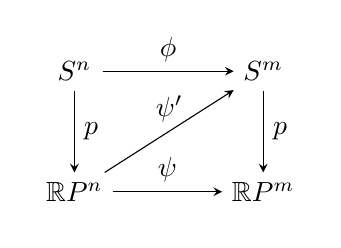
\begin{tikzpicture}
  \matrix (m) [matrix of math nodes,row sep=3em,column sep=4em,minimum width=2em] {
     S^n & S^m \\
     \mathbb{R}P^n & \mathbb{R}P^m \\};
  \path[-stealth]
    (m-1-1) edge node [right] {$p$} (m-2-1)
            edge  node [above] {$\phi$} (m-1-2)
    (m-2-1.east|-m-2-2) edge  node [above] {$\psi$} (m-2-2)
    (m-1-2) edge node [right] {$p$} (m-2-2)
            (m-2-1) edge  node [above]{$\psi'$} (m-1-2);
\end{tikzpicture}
\\
$\psi' \circ p$ and $\phi$ are both lifts of $\psi \circ p$ and both map $x\mapsto y$ so $\phi = \psi'\circ p$ by uniqueness. But then $\psi'(p(-x))=\psi'([x])=y=\phi(x)$, contradicting $\phi(-x)=-y$.
\end{proof}

\end{document}
